\documentclass[12pt]{article}
\usepackage{graphicx}
\usepackage{amsmath}
\usepackage{amssymb}
\usepackage{hyperref}
\usepackage {graphicx}
\usepackage{grffile}

\normalsize
\setlength{\hoffset}{0in} 
\setlength{\voffset}{0in}
\setlength{\oddsidemargin}{0in} 
\setlength{\topmargin}{0in}
\setlength{\headheight}{0in} 
\setlength{\headsep}{0in}
\setlength{\textheight}{9in} 
\setlength{\textwidth}{6.5in}
\setlength{\marginparsep}{0in} 
\setlength{\marginparwidth}{0in}
\setlength{\footskip}{24pt}
\setcounter{secnumdepth}{-1}


\newcommand{\beq}{\begin{equation}}
\newcommand{\eeq}{\end{equation}}
%\newcommand{\eps300}{$\epsilon$300}
%\newcommand{\eps4}{$\epsilon$ 4}

\begin{document}

\title{Foreground Separation with\\ GNILC and COMMANDER}
\author{Mathieu Remazeilles} 
\date{February, 2019} 
\maketitle

\begin{abstract}
\noindent We report on our map-based component separation results from sky simulations of the PICO experiment. We have implemented two different methods: a Bayesian parametric fitting algorithm, COMMANDER (Eriksen et al, ApJ 2008), and a blind ILC-type algorithm, GNILC (Remazeilles et al, MNRAS 2011).

\end{abstract}

\section{Map Simulations}
\label{sec:simulations}

\subsection{PySM}\label{subsec:pysm}

We have implemented GNILC on a series of sky simulations having different foreground models of increasing complexity, which have been generated by PySM software (Thorne et al, MNRAS 2017). The set of foreground models is similar to the one used by CMB-S4 Collaboration, but extrapolated to PICO frequencies, sensitivities, and resolutions. The series of PICO simulations is publicly available on the wiki\footnote{\url{https://zzz.physics.umn.edu/ipsig/20180424_dc_maps}}, and consists of several Galactic foreground models:

\begin{itemize}
\item PICO Report Model A / Model 90.92  / {\tt a2d4f1s3}: 

- Synchrotron power-law with curvature and variable spectral index over the sky (Kogut et al, ApJ 2012)

- Two thermal dust components, as the sum of two modified blackbodies with constant spectral indices but variable temperatures over the sky (Finkbeiner et al,  ApJ 1999)

- AME component with 2\% polarization

\item PICO Report Model B / Model 90.93 / {\tt a2d7f1s3}: 

- Synchrotron power-law with curvature and variable spectral index over the sky (Kogut et al, ApJ 2012)

- Hensley \& Draine's physical model of thermal dust (B. Hensley's PhD thesis, 2015) 

- AME component with 2\% polarization

\item PICO Report Model C / Model 90.96 / MHD: 

Thermal dust and synchrotron models derived from the MHD simulations of Kim, Choi \& Flauger (2019)

More detailed description (from Brandon Hensley): to get the synchrotron, we assumed a simple vertical profile for the cosmic ray electron distribution and a spatially uniform frequency dependence. The dust was implemented as simple modified blackbodies in every grid cell with temperatures based on the local radiation field (a simulation output) and a beta that was chosen based on the local gas density (the range of variation was kept quite small). This was then integrated up along the line of sight. The MHD simulations themselves are described in this recent paper cited above, and the dust model is described in Hensley's thesis: 
\begin{verbatim} 
https://search.proquest.com/openview/
8090d544e15c2afa47c1449c2b0e6048/1?pq-origsite=gscholar&cbl=18750&diss=y
\end{verbatim}
\end{itemize}

In addition to Galactic foregrounds, each simulation contains different realisations of the CMB signal and instrumental noise at PICO sensitivities. The CMB map realisations contain tensor modes at either $r=0$ or $r=3\times 10^{-3}$, and lensing modes at $A_L=1$ (100\% lensing contamination) or $A_L=0.15$ (85\% delensing). The simulated PICO frequency maps (21 maps ranging from $20$ to $800$\, GHz) thus include primordial CMB, lensing, Galactic foregrounds, and noise, and have been convolved with Gaussian beams at the resolutions quoted by the PICO experiment.


\subsection{PSM}\label{subsec:psm}

We have also considered another set of independent simulations based on the PSM software (Delabrouille et al 2013) for our COMMANDER analysis. The PSM simulations are generated at low resolution (HealPix $N_{\rm side}=16$) and contain primordial CMB B-modes at $r=10^{-3}$, full lensing B-modes ($A_L=1$), Galactic foregrounds, and instrumental noise at PICO sensitivities. Galactic foreground models in the PSM simulations consist of:

\begin{itemize}
\item Model PSM: 

- Synchrotron power-law with curvature and variable spectral index over the sky (Kogut et al, ApJ 2012)

- Thermal dust modified blackbody with variable spectral index and variable temperature over the sky (Planck intermediate results XLVIII, 2016)

\end{itemize}

Like the PySM simulations, the PSM map simulations consist of 21 PICO maps ranging from $20$ to $800$\, GHz which have been convolved with Gaussian beams at the resolutions quoted by the PICO experiment 


\section{Analysis with COMMANDER}

COMMANDER (Eriksen et al, ApJ 2008) is a Bayesian parametric method for multi-component spectral fitting using Gibbs sampling. A spectral model for all the components of emission is fitted in each pixel. We implement COMMANDER to perform component separation and CMB B-mode power spectrum reconstruction, and use a Blackwell-Rao likelihood to estimate the tensor-to-scalar ratio $r$ from the recovered CMB B-mode power spectrum after foreground cleaning.

We first report on the COMMANDER results on the PSM simulations by considering two configurations of PICO (Fig.~\ref{Fig:commander_pico_90p91}): the \emph{baseline} version with a broad frequency range of {$20$-$800$\,GHz}, and a \emph{descoped} version with a narrower frequency of {$43$-$462$\,GHz} where we discarded low- and high-frequency channels in the component separation analysis.

%%%%%%%%%%%%%%%%%%%%%%%%%%%%%%%%%%%%%%%%%%%%%%%%%%%%%%
\begin{figure}
  \begin{center}
    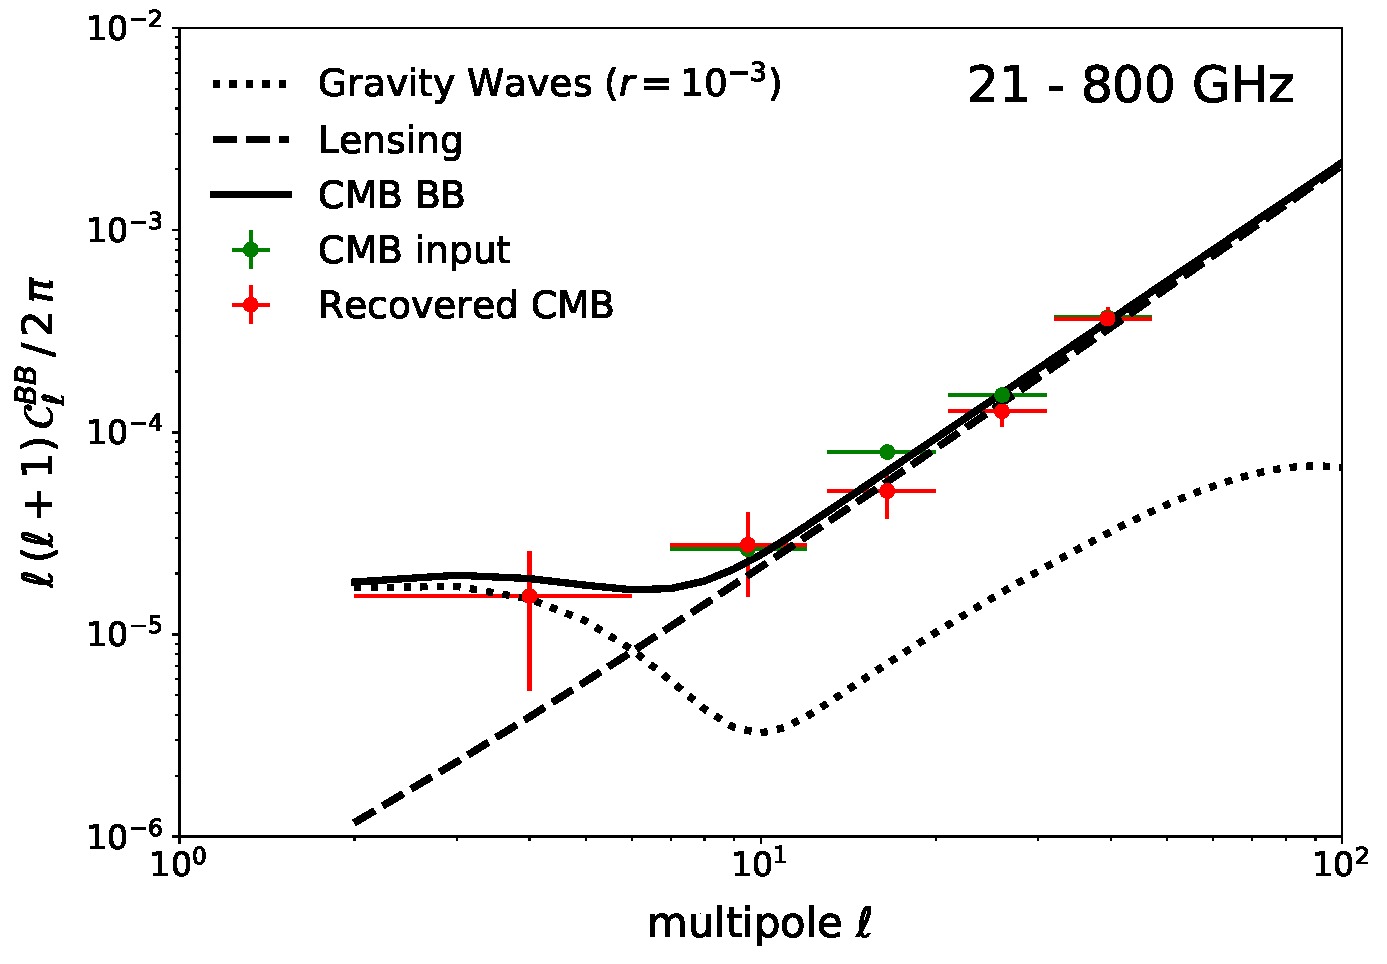
\includegraphics[width=0.5\columnwidth]{figures_memo/commander_pico_baseline.pdf}~
     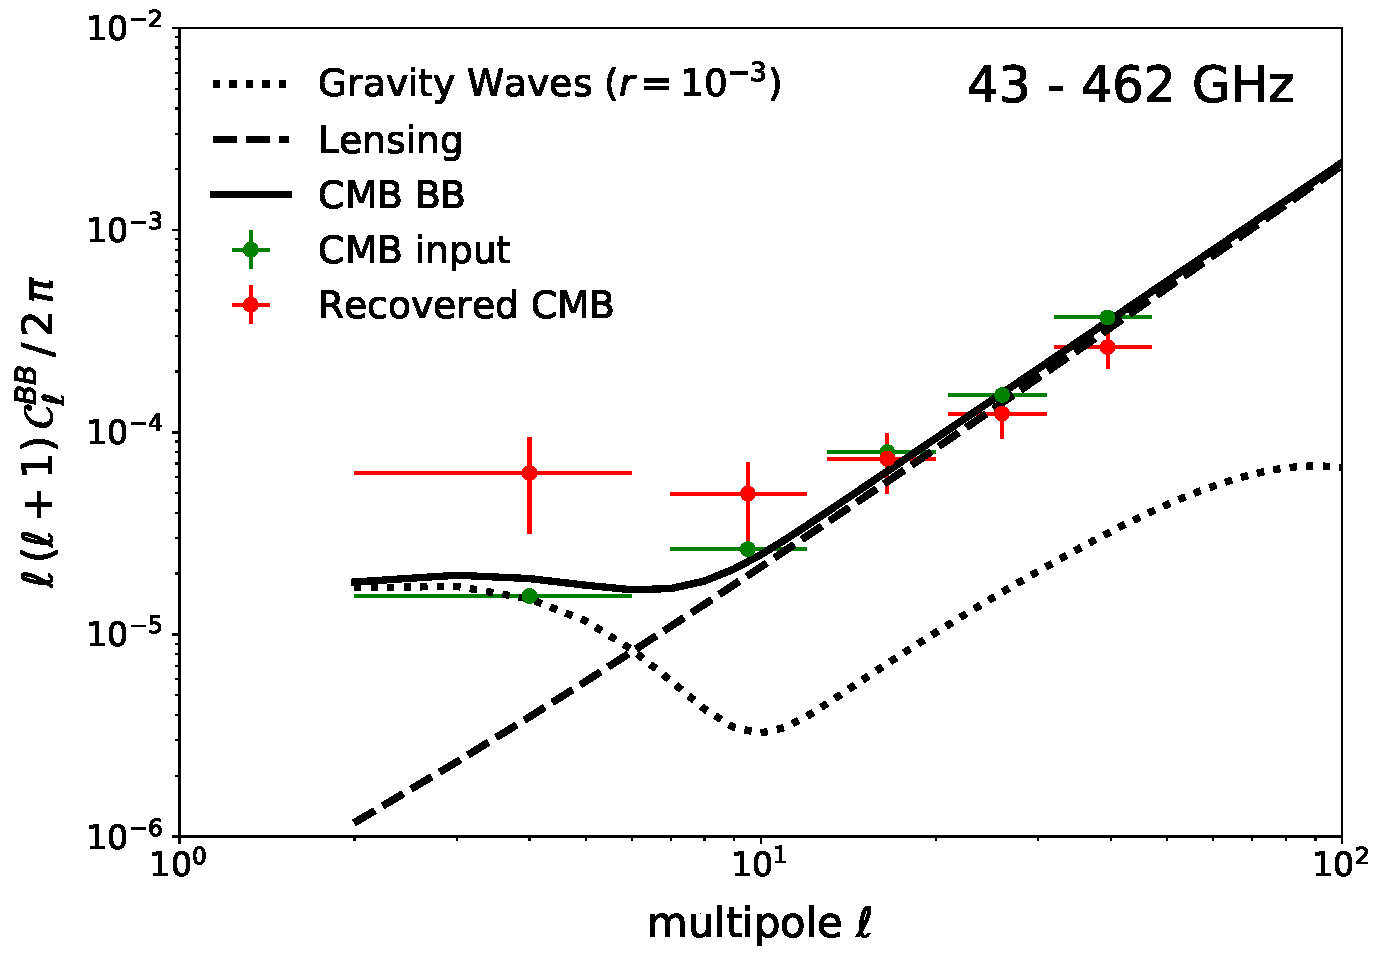
\includegraphics[width=0.5\columnwidth]{figures_memo/commander_pico_descoped.pdf}~
  \end{center}
\caption{Reconstruction of the CMB B-mode power spectrum with COMMANDER after foreground removal on $f_{sky}=50\%$ of the sky for the PICO baseline configuration (\emph{left}) and a descoped version of PICO (\emph{right}): primordial B-modes at $r=10^{-3}$ (\emph{dotted black}); lensing B-modes (\emph{dashed black}); CMB B-modes (\emph{solid black}); CMB B-mode input realisation (\emph{green dots}); and recovered CMB B-mode with COMMANDER (\emph{red dots}). {\bf This figure has been included in the PICO report.}}
\label{Fig:commander_pico_90p91}
\end{figure}
%%%%%%%%%%%%%%%%%%%%%%%%%%%%%%%%%%%%%%%%%%%%%%%%%%%%%%

For the baseline configuration of PICO ({$20$-$800$\,GHz}; left panel of Fig.~\ref{Fig:commander_pico_90p91}), COMMANDER is able to remove Galactic foregrounds to the desired accuracy and reconstruct the CMB B-mode power spectrum at large angular scales ($2\leq \ell \lesssim 50$). When narrowing the frequency range of observations by PICO to {$43$-$462$\,GHz} (right panel of Fig.~\ref{Fig:commander_pico_90p91}), the recovered CMB B-modes by COMMANDER are biased towards the largest angular scales due to residual foreground contamination.

To understand the source of the bias on the CMB reconstruction for the descoped version of PICO, one can have a look at the reconstructed foreground spectral parameters by COMMANDER (Fig.~\ref{Fig:commander_pico_90p91_foregrounds}). The absence of of high frequencies $> 462$\,GHz would prevent a descoped version of PICO from constraining the dust temperature with the desired accuracy (bottom right panel of Fig.~\ref{Fig:commander_pico_90p91_foregrounds}). Extrapolating the error on the reconstructed dust temperature over the sky towards CMB frequencies translates into a bias on the reconstructed CMB B-mode power spectrum at large angular scales due to residual dust contamination at a level of $\Delta r > 10^{-3}$ (right panel of Fig.~\ref{Fig:commander_pico_90p91}).

%%%%%%%%%%%%%%%%%%%%%%%%%%%%%%%%%%%%%%%%%%%%%%%%%%%%%%
\begin{figure}
  \begin{center}
 %   \includegraphics[width=\columnwidth]{u}~\\
    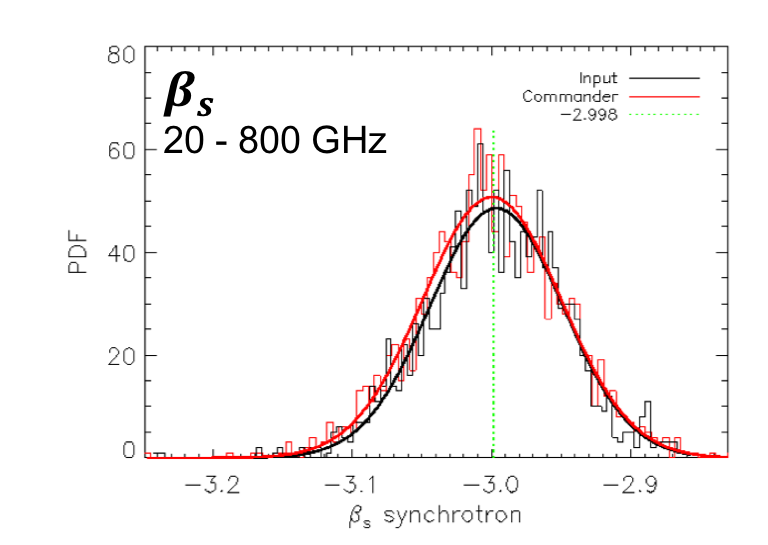
\includegraphics[width=0.33\columnwidth]{figures_memo/beta_synch_baseline.png}~
     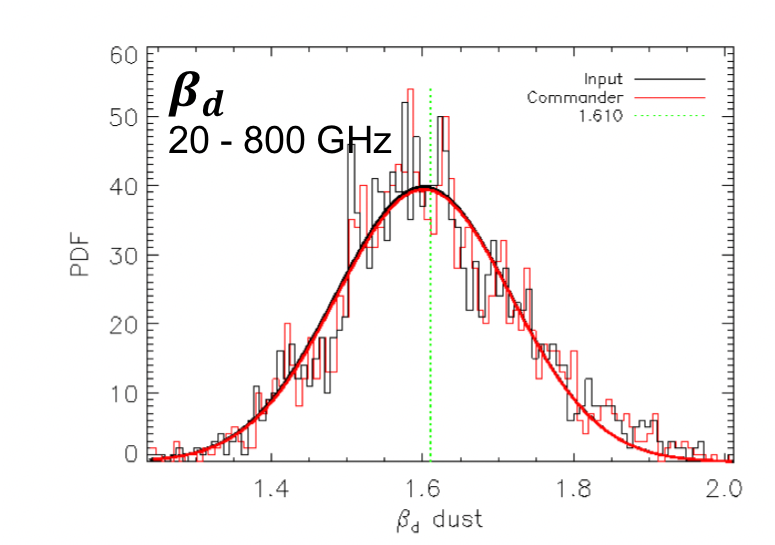
\includegraphics[width=0.33\columnwidth]{figures_memo/beta_dust_baseline.png}~
     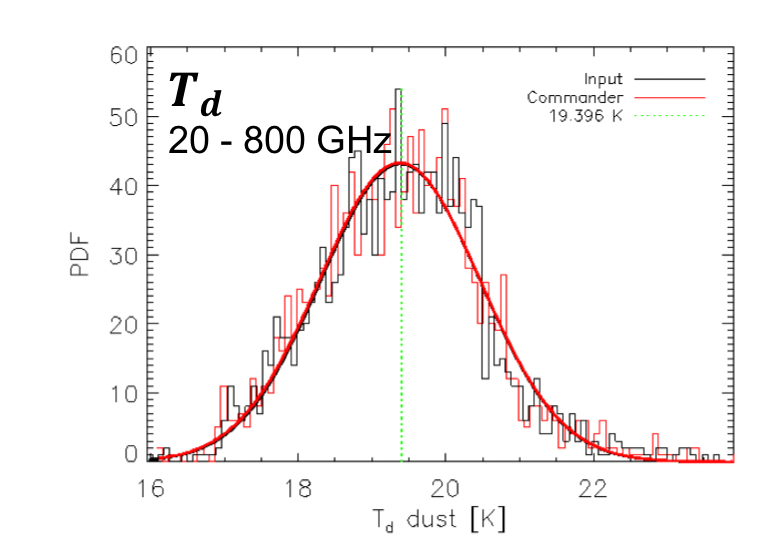
\includegraphics[width=0.33\columnwidth]{figures_memo/temperature_dust_baseline.png}~\\
     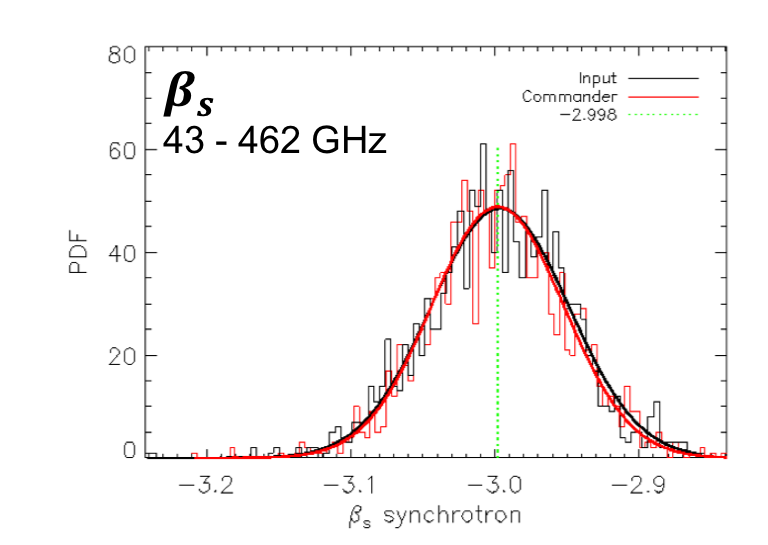
\includegraphics[width=0.33\columnwidth]{figures_memo/beta_synch_descoped.png}~
     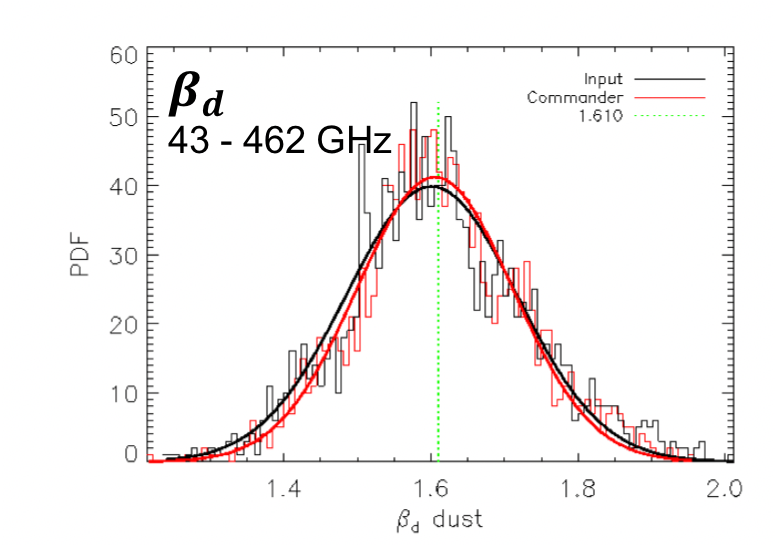
\includegraphics[width=0.33\columnwidth]{figures_memo/beta_dust_descoped.png}~
     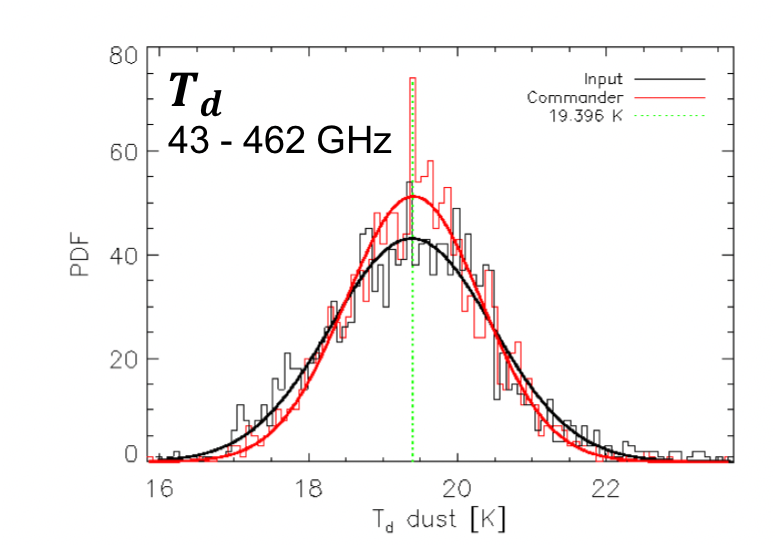
\includegraphics[width=0.33\columnwidth]{figures_memo/temperature_dust_descoped.png}~
  \end{center}
\caption{Reconstruction (\emph{red}) of the distribution over the sky of foreground spectral parameters (\emph{black}) with COMMANDER for the PICO baseline configuration (\emph{top}) and a descoped version of PICO (\emph{bottom}): synchrotron spectral index (\emph{left}); dust spectral index (\emph{middle}); and dust temperature (\emph{right}). The absence of high frequencies $> 462$\,GHz would prevent PICO from constraining the dust temperature with the desired accuracy (\emph{bottom right panel}).}
\label{Fig:commander_pico_90p91_foregrounds}
\end{figure}
%%%%%%%%%%%%%%%%%%%%%%%%%%%%%%%%%%%%%%%%%%%%%%%%%%%%%%

The recovered probability distribution of tensor-to-scalar ratio by COMMANDER for the PICO baseline configuration ({$20$-$800$\,GHz}) is $r=(0.51\pm0.36)\times 10^{-3}$ (Fig.~\ref{Fig:commander_pico_90p91_r_baseline}), based on a \emph{single} realisation, hence about $3\sigma$ detection of $r=10^{-3}$ in the absence of delensing. After foreground cleaning and 60\% delensing, the significance of the detection of $r=10^{-3}$ by PICO increases to $4\sigma$ with $\sigma(r=10^{-3})=0.24\times 10^{-3}$.

%%%%%%%%%%%%%%%%%%%%%%%%%%%%%%%%%%%%%%%%%%%%%%%%%%%%%%
\begin{figure}
  \begin{center}
     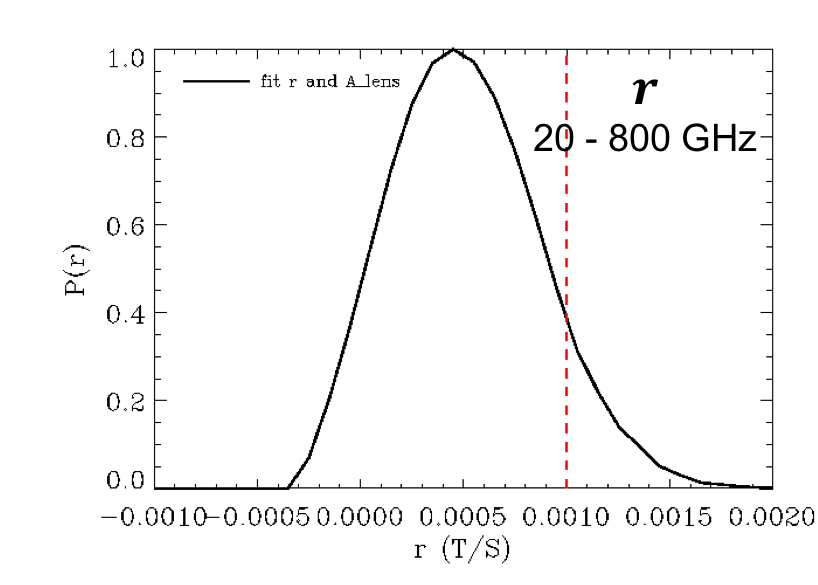
\includegraphics[width=0.5\columnwidth]{figures_memo/tensor_to-scalar_baseline.png}~
  \end{center}
\caption{Recovered distribution of the tensor-to-scalar ratio after foreground removal by COMMANDER for the PICO baseline configuration (single realisation). The uncertainty on the tensor-to-scalar ratio is of $\sigma(r=10^{-3})=0.36\times 10^{-3}$. }
\label{Fig:commander_pico_90p91_r_baseline}
\end{figure}
%%%%%%%%%%%%%%%%%%%%%%%%%%%%%%%%%%%%%%%%%%%%%%%%%%%%%%

\section{Analysis with GNILC}

GNILC (Remazeilles et al, MNRAS 2011) is blind component separation method which does not rely on any modelling of the foregrounds. GNILC is implemented on a needlet (spherical wavelet) frame, whose localization properties in both pixel space and harmonic space allows to adapt the component separation to the local conditions of contamination both over the sky and over the angular scales. The idea behind GNILC is to first look for the \emph{independent} (not physical) foreground degree of freedom locally over the sky and over the angular scales in order to identify the local dimensionality of the foreground subspace. This is enabled through a prior on the instrumental noise covariance matrix that is compared to the full data covariance matrix in a principal component analysis. Then, the data are projected onto the local foreground subspaces (data compression) to get rid of the noise, and an ILC is performed in the foreground subspace, allowing GNILC to focus variance minimization in the foreground subspace instead of minimizing the variance of noise plus foregrounds.

We report on the GNILC results on the series of PySM simulations (model 90.92 / A, model 90.93 / B, and model 90.96 / C) by considering the baseline PICO configuration  ({$20$-$800$\,GHz}). 

\subsection{Main results: $r=0$, $A_L=0.15$}

Our GNILC results for the fiducial values $r=0$ and $A_L=0.15$ (no tensor modes, 85\% delensing) are shown in Fig.~\ref{Fig:gnilc_ps_r0_AL0p15} for the different foreground models of the PICO PySM simulations. Our results are averaged over 6 different realisations of the CMB and noise in the simulations. For each foreground model, the fiducial CMB B-mode power spectrum ($r=0$, \emph{dashed black}) is recovered by GNILC on a broad range of multipoles (\emph{solid red}), while the residual foregrounds (\emph{dotted orange}) are  reduced by GNILC below the typical level of primordial CMB B-modes at $r=5\times 10^{-4}$ over the multipoles $2 \leq \ell \lesssim 200$  . 

Figure ~\ref{Fig:gnilc_ps_residuals_all_models} shows that GNILC is pretty robust and insensitive to the complexity of the foregrounds, with the residual foreground contamination being controlled at a level below $r=5\times 10^{-4}$ consistently for all the foreground models.

%%%%%%%%%%%%%%%%%%%%%%%%%%%%%%%%%%%%%%%%%%%%%%%%%%%%%%
\begin{figure}
  \begin{center}
    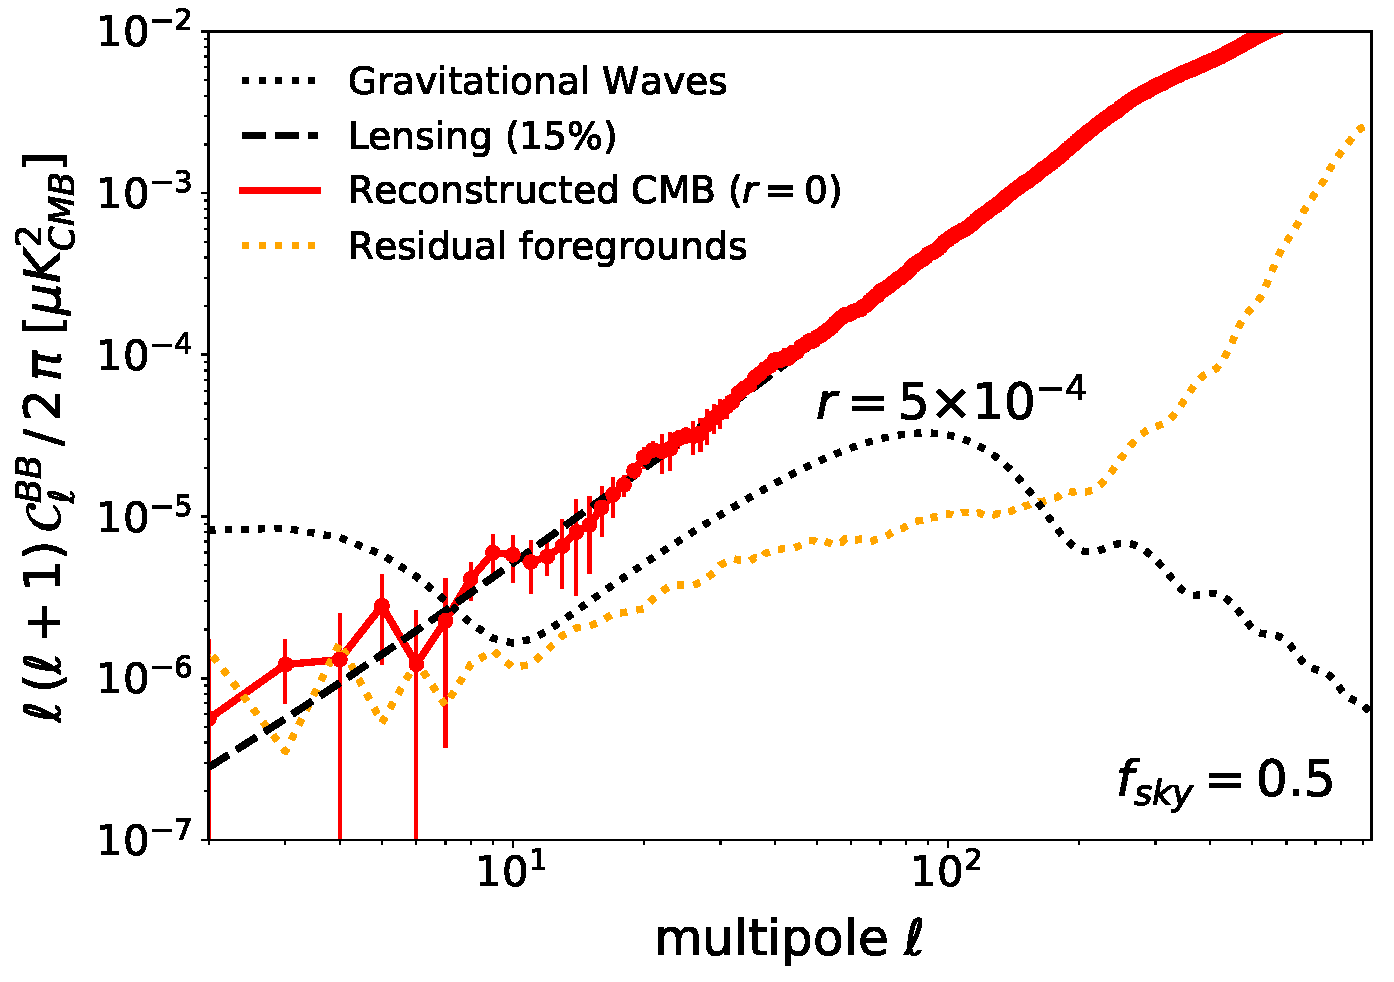
\includegraphics[width=0.33\columnwidth]{figures_memo/gnilc_pico_90p92_r0_AL0p15_mc_test3_final.pdf}~
     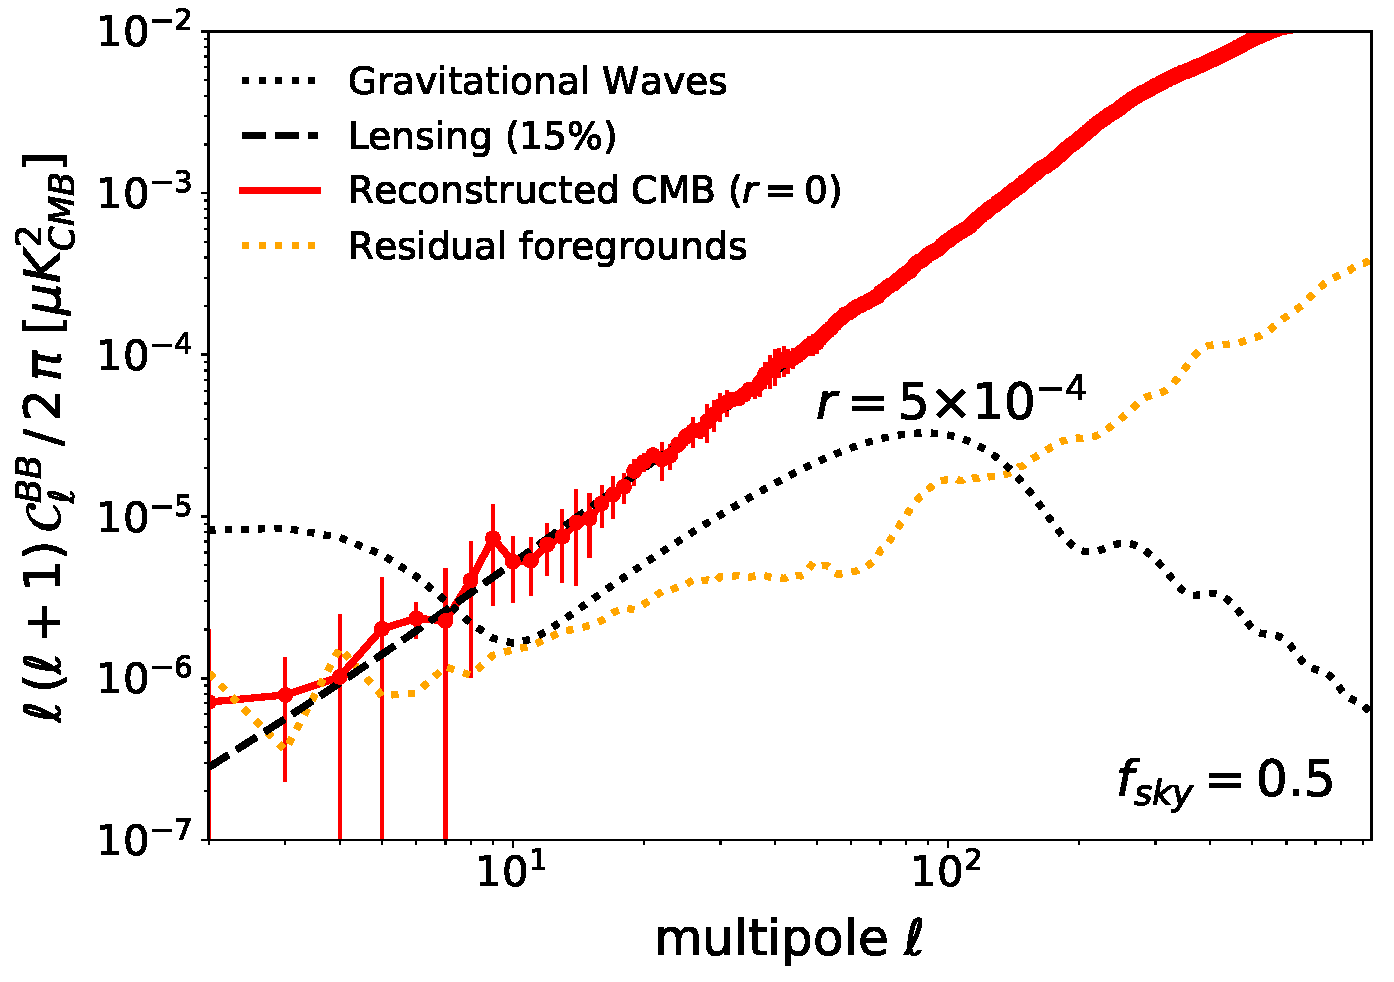
\includegraphics[width=0.33\columnwidth]{figures_memo/gnilc_pico_90p93_r0_AL0p15_mc_test3_final.pdf}~
     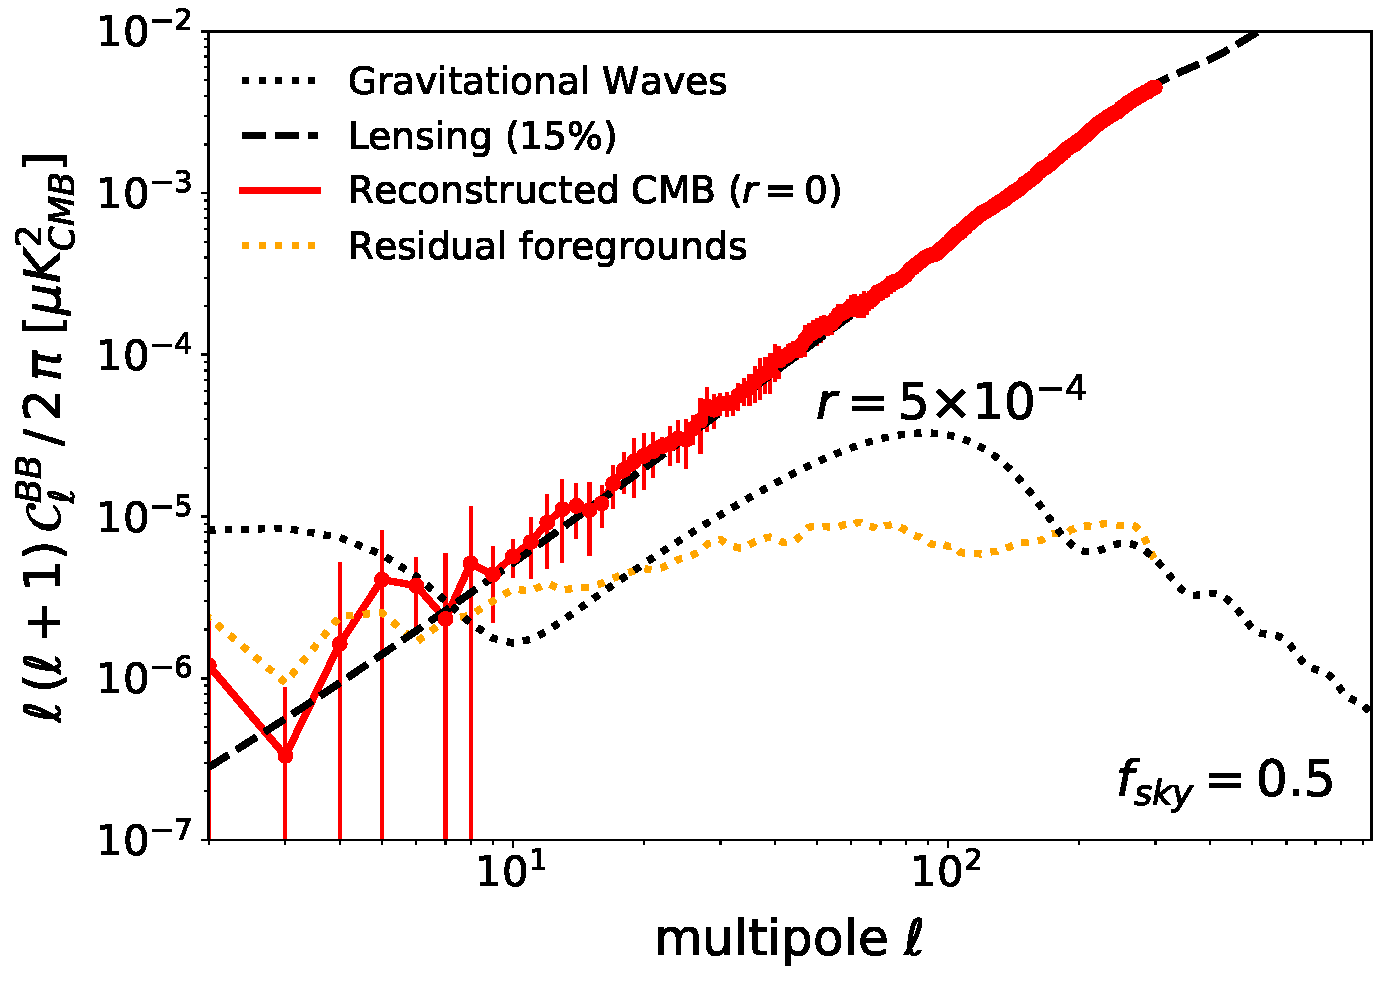
\includegraphics[width=0.33\columnwidth]{figures_memo/gnilc_pico_90p96_r0_AL0p15_mc_test3_final.pdf}~	
  \end{center}
\caption{Reconstruction of the CMB B-mode power spectrum with GNILC after foreground removal on $f_{sky}=50\%$ of the sky for the PICO baseline configuration and for different foreground models: model 90.92 (model A; \emph{left}), model 90.93 (model B; \emph{middle}), and model 90.96 (model C; \emph{right}). The fiducial value of the tensor-to-scalar ratio is $r=0$ (no primordial B-mode), while $A_L=0.15$ to account for 85\% delensing. These results are for 6 independent realisations of the CMB and noise. {\bf Left panel has been included in the PICO report.}}
\label{Fig:gnilc_ps_r0_AL0p15}
\end{figure}
%%%%%%%%%%%%%%%%%%%%%%%%%%%%%%%%%%%%%%%%%%%%%%%%%%%%%%

%%%%%%%%%%%%%%%%%%%%%%%%%%%%%%%%%%%%%%%%%%%%%%%%%%%%%%
\begin{figure}
  \begin{center}
    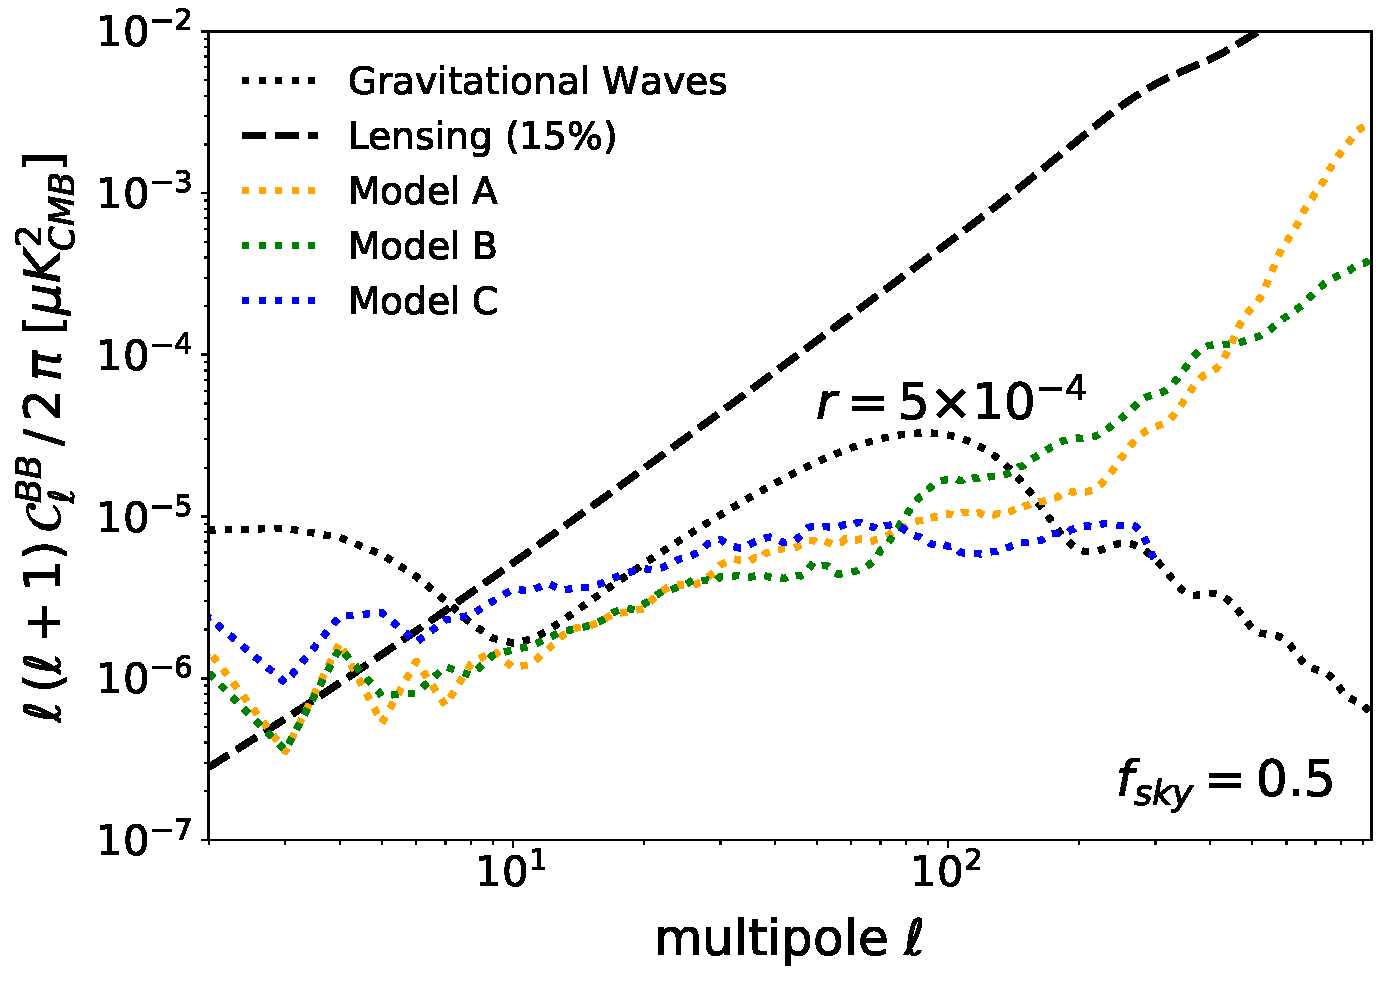
\includegraphics[width=0.5\columnwidth]{figures_memo/gnilc_pico_allmodels_r0_AL0p15_mc_test3_final.pdf}~
   \end{center}
\caption{Power spectrum of residual foregrounds after component separation with GNILC for different foreground models: model A / 90.92 (\emph{dotted orange}),  model B / 90.93 (\emph{dotted green}), and model C / 90.96 (\emph{dotted blue}). {\bf This figure has been included in the PICO report.}}
\label{Fig:gnilc_ps_residuals_all_models}
\end{figure}
%%%%%%%%%%%%%%%%%%%%%%%%%%%%%%%%%%%%%%%%%%%%%%%%%%%%%%

\subsection{Earlier results: $r=3\times 10^{-3}$, $A_L=1$}

We have also considered a set of PICO PySM simulations having tensor modes at ${r=3\times 10^{-3}}$ and full lensing contamination at ${A_L=1}$, i.e. without delensing. The GNILC results on the reconstruction of the CMB B-mode power spectrum in this case are shown in Fig.~\ref{Fig:gnilc_ps_r0p003_AL1}. {\bf Note that the following results were produced earlier in the analysis, when the GNILC algorithm was not yet optimized, so that the most relevant results are still those shown above for $\boldsymbol{r=0}$ and $\boldsymbol{A_L=0.15}$}. 
%%%%%%%%%%%%%%%%%%%%%%%%%%%%%%%%%%%%%%%%%%%%%%%%%%%%%%
\begin{figure}
  \begin{center}
    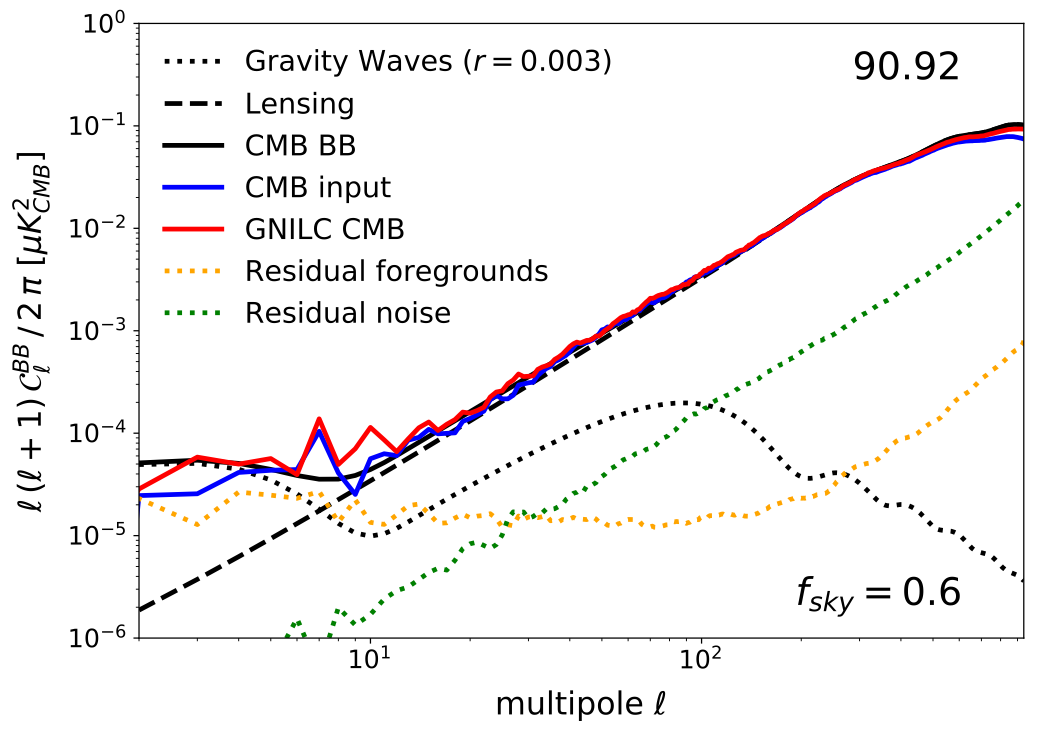
\includegraphics[width=0.33\columnwidth]{figures_memo/gnilc_pico_90p92_r0p003_AL1.png}~
     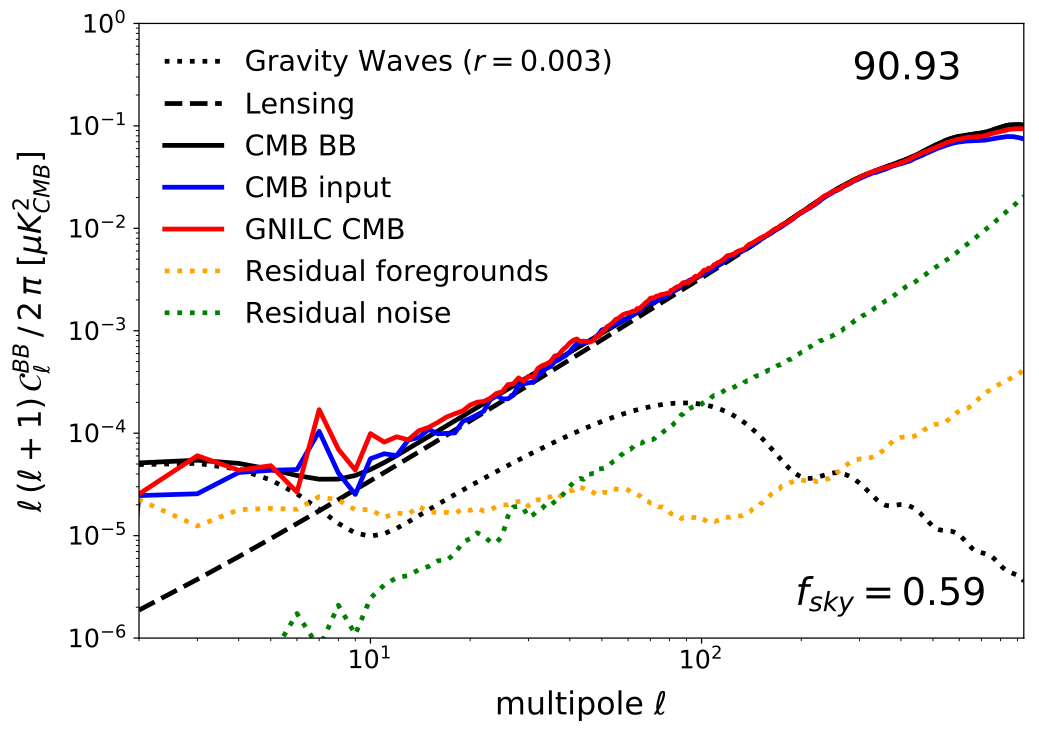
\includegraphics[width=0.33\columnwidth]{figures_memo/gnilc_pico_90p93_r0p003_AL1.png}~
     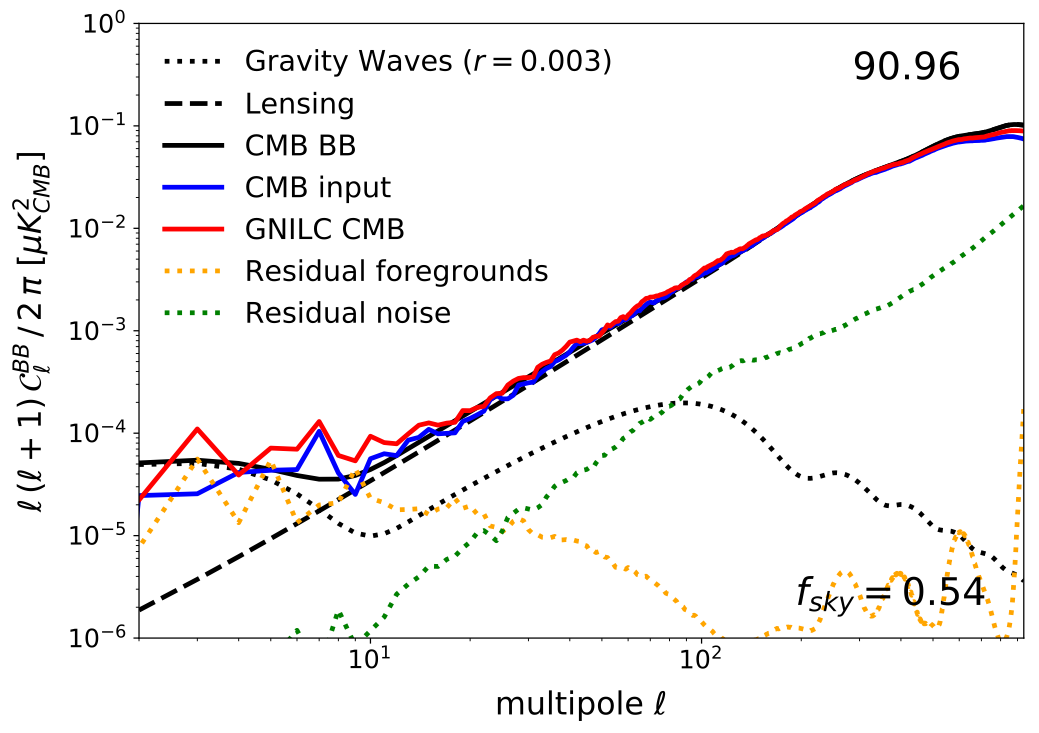
\includegraphics[width=0.33\columnwidth]{figures_memo/gnilc_pico_90p96_r0p003_AL1.png}~	
  \end{center}
\caption{Reconstruction of the CMB B-mode power spectrum with GNILC after foreground removal for $r=3\times 10^{-3}$, while $A_L=1$ (no delensing) and for different foreground models of the PICO simulations: model 90.92 (model A; \emph{left}), model 90.93 (model B; \emph{middle}), and model 90.96 (model C; \emph{right}). The various power spectra are: fiducial tensor B-modes at $r=3\times 10^{-3}$ (\emph{dotted black}), fiducial lensing B-modes at $A_L=1$ (\emph{dashed black}), fiducial CMB B-modes (\emph{solid black}), CMB B-mode input realisation (\emph{solid blue}), recovered CMB B-modes by GNILC (\emph{solid red}), residual foregrounds (\emph{dotted orange}), and residual noise (\emph{dotted green}).}
\label{Fig:gnilc_ps_r0p003_AL1}
\end{figure}
%%%%%%%%%%%%%%%%%%%%%%%%%%%%%%%%%%%%%%%%%%%%%%%%%%%%%%



%\section{Results}



\end{document}



